\documentclass[11pt,letterpaper]{article}
\usepackage[T1]{fontenc}
\usepackage{lmodern}
\ifdefined\pdfgentounicode
  \input{glyphtounicode}
  \pdfgentounicode=1
\fi
\usepackage[margin=1.1in,marginparwidth=.88in,marginparsep=.12in]{geometry}
\usepackage{amsmath,amssymb,amsthm}
\usepackage{microtype,xcolor,mdframed,marginnote,ragged2e}
\usepackage{tikz}
\usepackage{hyperref}
\definecolor{linkblue}{RGB}{25,65,100}
\definecolor{notegray}{RGB}{76,76,76}
\hypersetup{colorlinks=true,linkcolor=linkblue,citecolor=linkblue,urlcolor=linkblue,
  pdftitle={VP versus VNP over every field},
  pdfsubject={A geometric lower bound for weighted clique}}
\newtheorem{theorem}{Theorem}[section]
\newtheorem{lemma}[theorem]{Lemma}
\newtheorem{proposition}[theorem]{Proposition}
\newtheorem{corollary}[theorem]{Corollary}
\newtheoremstyle{importstyle}{0pt}{0pt}{\normalfont}{}{\bfseries}{.}{.5em}{}
\theoremstyle{importstyle}
\newtheorem{imported}{Imported Theorem}
\renewcommand{\theimported}{\Alph{imported}}
\newmdenv[linecolor=linkblue,linewidth=.7pt,innerleftmargin=10pt,
  innerrightmargin=10pt,innertopmargin=8pt,innerbottommargin=8pt,
  skipabove=.8\baselineskip,skipbelow=.8\baselineskip,nobreak=true]{importbox}
\newcommand{\F}{F}
\newcommand{\VP}{\mathrm{VP}}
\newcommand{\VNP}{\mathrm{VNP}}
\newcommand{\Clique}{\operatorname{Clique}}
\renewcommand{\marginfont}{%
  \normalfont\fontsize{8}{9.5}\selectfont
  \color{notegray}\hypersetup{allcolors=notegray}}
\renewcommand{\raggedrightmarginnote}{%
  \setlength{\RaggedRightRightskip}{0pt plus 1.6em}%
  \RaggedRight\pretolerance=-1\relax}
\newcommand{\sourcenote}[1]{\marginnote{#1}}
\newcommand{\paperat}[2]{\href{https://github.com/anthropics/formal-math/blob/918c8e2778aee18b0283dc5a33ed39ab3cd63a96/vp-vnp/paper.pdf\#page=#1}{#2}}
\newcommand{\wire}{\mathsf W}
\newcommand{\bal}{\mathcal B}
\newcommand{\norm}[1]{\lVert#1\rVert}
\newcommand{\inner}[2]{\langle#1,#2\rangle}
\title{\(\VP\) versus \(\VNP\) over every field}
\author{}
\date{November 25, 2026}
\AddToHook{cmd/maketitle/after}{%
  \par\noindent\begin{minipage}{\linewidth}
  \small\sffamily
  I asked ChatGPT these questions to understand what follows from the recent
  VP versus VNP breakthrough. I share its answers so that these explorations
  are available beyond a private conversation. These are AI-generated notes,
  not research papers. I do not claim authorship or priority for the ideas.
  Arguments may be wrong, and earlier work may be overlooked or misattributed.
  I welcome corrections by mail or via
  \href{https://github.com/radomite/algebraic-complexity/issues}{GitHub}.
  \end{minipage}\par\medskip
}
\AddToHook{shipout/foreground}{%
  \ifnum\ReadonlyShipoutCounter>1\relax
  \put(0pt,-24pt){\makebox[\paperwidth][c]{%
    \normalfont\sffamily\fontsize{8}{10}\selectfont\color[gray]{0.38}%
    AI-generated exploration notes. Arguments and attributions may be wrong.
    \href{https://github.com/radomite/algebraic-complexity/issues}{Corrections welcome on GitHub.}}}%
  \fi
}

\begin{document}
\maketitle

Fix a field \(F\). Give each vertex and edge of a graph its own weight.
The weight of a clique is the product of the weights of its vertices and
edges. We show that the polynomial adding up all these weights belongs to
\(\VNP_F\) and requires more than polynomial-size arithmetic circuits.
Thus \(\VP_F\subsetneq\VNP_F\).

The proof follows the cliques of a fixed order \(k\). A small circuit
would express the clique sum as a sum of networks. In each network
two groups of vertices communicate through a narrow wire joining two hubs. We draw the wires in Euclidean space, where a theorem of
OpenAI assigns a cost to each bit sent between two points. Moving the
hubs a short distance apart shows how many bits their connecting wire
must carry. As \(k\) grows, this gives a growing lower bound on the
exponent of the circuit size in the number of vertices. It also separates
the parameterized classes \(\mathrm{VFPT}_F\) and \(\mathrm{VW}[1]_F\).

The sole imported result is the existence of Euclidean wire prices,
stated in Section~\ref{sec:prices}. We derive the circuit decomposition,
the geometric estimate, and both class separations below.

\section{Clique polynomials and tensors}
\label{sec:cliques}

Write \([N]=\{1,\ldots,N\}\). Give the vertices of the complete graph
on \([N]\) variables \(X_i\), and give
each edge \(\{i,j\}\) a variable \(E_{ij}\), with \(i<j\).
The weighted-clique polynomial is%
\sourcenote{Vertex and edge weights follow Bläser and Engels~\cite{be}.}
\[
 \Clique_N(X,E)=\sum_{U\subseteq[N]}
       \prod_{i\in U}X_i\prod_{\substack{i,j\in U\\i<j}}E_{ij}.
\]
Setting $E_{ij}\gets 0$ removes every clique using edge $ij$.
Write \(\Clique_{N,k}\) for the part of this sum using exactly \(k\) vertices.
A choice of \(N\) bits specifies a subset, and its weight can be computed
with polynomially many field operations. Summing over the choices puts
\((\Clique_N)\) in \(\VNP_F\) (Appendix~\ref{app:selectors}).

We use \(\Clique_{N,k}\) to express a polynomial on the complete graph \(K_k\),
where \(k\ge2\). Give each edge a label from \([q]=\{1,\ldots,q\}\).
For a labelling \(\sigma\), let \(\sigma_i\) be the tuple of labels
seen at vertex \(i\), in order of the other endpoints. Put
\[
      Z_{k,q}=\sum_{\sigma:E(K_k)\to[q]}\ \prod_{i=1}^k x_{i,\sigma_i}.
\]
For a triangle this is \(\sum_{a,b,c}x_{1,(a,b)}x_{2,(a,c)}x_{3,(b,c)}\).
Each label appears at both ends of its edge. The alphabet can grow
because its symbols index variables over \(\F\).

\begin{lemma}\label{lem:colors}
For \(N=kq^{k-1}\), setting some variables of \(\Clique_{N,k}\) to zero
or one and renaming the others gives \(Z_{k,q}\).
\end{lemma}
\begin{proof}
Make one color class for each vertex \(i\) of \(K_k\). Its \(q^{k-1}\)
vertices are the possible tuples \(\rho\) of labels at \(i\), and the
vertex for \(\rho\) gets weight \(x_{i,\rho}\). Give edges within a color
weight zero. Between colors \(i\) and \(j\), give an edge weight one
if the two tuples agree on the label of \(ij\), and zero otherwise.
A surviving \(k\)-clique uses each color once. Its tuples specify one
labelling of the complete graph, and every labelling occurs exactly once.
\end{proof}

\section{Geometry of wires}
\label{sec:prices}

An \emph{equality wire} between distinct sites \(u,v\) carries a label
from \([q]\). Its entry is one when the labels at its ends agree and zero
otherwise. In the standard basis its tensor is
\[
   \wire_{uv}(q)=\sum_{i=1}^q e_i\otimes e_i,
\]
with the first factor at \(u\) and the second at \(v\).
At a triangle of sites, put a binary wire on each edge. Its three bits
can be chosen independently. If the triangle has perimeter \(P\), the
geometry theorem assigns these wires total cost \(P\). There is also a
tensor with just one bit copied to all three sites. Its only nonzero
entries are at \(000\) and \(111\). That tensor costs \(P/2\). In
\(Z_{k,q}\) each edge has its own label, as in the first example. We
will use the following part of the theorem.

\begin{importbox}
\begin{imported}\label{imp:geometry}
Place finitely many sites in Euclidean space, with at least two distinct
positions. Over any field there is a spectral point \(\phi\) and a scale
\(c>0\) such that, simultaneously for every binary wire,
\[
        c\log_2\phi(\wire_{uv}(2))=\norm{u-v}.
\]
\end{imported}
\end{importbox}

Here \(\phi\) assigns a number to each tensor on the sites. Its values
multiply on tensor products. If a tensor is the sum of local linear
images of several tensors, its value is at most the sum of theirs
(Appendix~\ref{app:tensors}). A wire with \(q=2^\ell\) labels is a
bundle of \(\ell\) binary wires. Two labels agree exactly when all their
bits agree. Its cost \(c\log_2\phi(\wire_{uv}(q))\) is therefore
\(\ell\norm{u-v}\).

\paragraph*{Where the theorem comes from.}
OpenAI proves that, over each field, wire prices realize Euclidean
spaces of arbitrarily large finite dimension.%
\sourcenote{OpenAI~\cite{euclid}, Theorems 1.1 and 1.2. The triangle is
Figure 1.}
The proof supposes there is a largest such dimension. The missing
higher-dimensional cube then gives a way to simulate many copies of a
computation with fewer wires per copy. The authors use the space saved
to run the simulator inside the original computation. They arrange for
the two outputs to differ by exactly the tensor their error bound excludes. We use the resulting existence theorem on one finite
drawing at a time. The companion note \href{../ports/ports.pdf}{\emph{When Does a Field Have Ports?}} starts from these Euclidean prices and asks whether a bounded-degree graph can control average squared wire cost for every placement the field admits.

\section{What a small circuit would have to send}
\label{sec:flat}

Fix \(k\ge2\) and take \(q=2^\ell\). Let \(L_\ell\) be the smallest
circuit size for \(Z_{k,q}\). We count all gates, including inputs,
with field constants and binary addition and multiplication. We relate \(L_\ell\) to a distance in
a Euclidean drawing of the complete graph.%
\sourcenote{The wire argument follows Anthropic, Appendices A and E. See the drawing in \paperat{33}{Proposition E.5}.}

\subsection*{A circuit gives two hubs for each balanced cut}

Think of the variables at vertex \(i\) as one block \(x_i\).
Every monomial of \(Z_{k,q}\) uses one variable from each block.
Call \(S\subseteq[k]\) balanced if \(k/3\le |S|\le 2k/3\), and
write \(\bal\) for these sets.

\begin{lemma}[Balanced products]\label{lem:balanced}
A size-\(L\) circuit for \(Z_{k,q}\) gives a decomposition
\begin{equation}
 Z_{k,q}=\sum_{S\in\bal}\sum_{j=1}^{L}
              g_{S,j}(x_S)\,h_{S,j}(x_{\bar S}), \qquad
              \bar S=[k]\setminus S .
 \label{eq:balanced}
\end{equation}
Each factor uses exactly one variable from each of its indicated
blocks in every monomial.
\end{lemma}

\begin{proof}
Let \([P]_U\) denote the component using one variable from
each block of \(U\) and zero from the other blocks. At a product gate,
\([AB]_U=\sum_{V\sqcup W=U}[A]_V[B]_W\), with ordered splits.
Starting at \(U=[k]\), follow the larger side of each split, breaking
ties to the left, as long as \(|U|>2k/3\). This side always has more
than \(k/3\) blocks. At an addition, expand both summands. An input
gate has zero component on more than \(2k/3\) blocks. Thus each
nonzero term stops at a gate \(g\) on a balanced set \(S\).
Its factor there is always \([P_g]_S\), and everything accumulated
beside it uses precisely the complementary blocks. Collecting by
\((g,S)\) gives~\eqref{eq:balanced}, with at most \(L\) choices of
\(g\) for a given \(S\).
\end{proof}

Now split the tuple index at vertex \(i\) into its individual labels,
identifying \(e_\rho\) with \(\bigotimes_{j\ne i}e_{\rho(j)}\).
Each ordered edge end \((i,j)\) has its own index. The coefficient
array of \(Z_{k,q}\) has a one exactly when the two labels
on every edge agree. The tensor is therefore a product of
\(\binom{k}{2}\) equality wires, one per edge. Call this the target.
For a cut \(S\), place a hub on each side. Connect every end to the hub
on its side by a \(q\)-dimensional wire, and connect the two hubs by
a wire of dimension \(2^{r_\ell}\), where \(r_\ell=\lceil\log_2 L_\ell\rceil\) for a smallest circuit.
The network tensor is the \(\boxtimes\)-product of these wires.

Apply Lemma~\ref{lem:balanced} to a circuit of size \(L_\ell\).
The network for \(S\) covers the inner sum in~\eqref{eq:balanced} by
one restriction. The middle wire supplies the same index \(j\) to
both hubs. The linear functional at the first hub reads \(j\) and the
labels at the ends on its side, and returns the corresponding coefficient
of \(g_{S,j}\). The other hub does this for \(h_{S,j}\). Unused
indices give zero. Summing over the middle label gives exactly the
inner sum. Use a separate pair of hubs for each \(S\), with
one-dimensional factors at unused sites. These networks together cover
the target.

\subsection*{A Euclidean drawing forces the middle wire to be large}

\begin{proposition}\label{prop:wire}
For each fixed \(k\ge2\), the circuit-size exponent in the alphabet size
satisfies
\[
   \beta:=\liminf_{\ell\to\infty}\frac{\log_2 L_\ell}{\ell}
                      \ \ge\ \frac{k^{3/2}}{3}.
\]
\end{proposition}
\begin{proof}
Put the end \((i,j)\) at the unit vector
\(u_{ij}=(e_i-e_j)/\sqrt2\) in \(\mathbb R^k\).
Opposite ends are at opposite vectors, so their total length is \(2m\) for
\(m=\binom{k}{2}\). The vector sum on the side of a cut \(S\) is
\[
  v_S=\sum_{i\in S,\ j\ne i}u_{ij},\qquad
  \norm{v_S}^2=\frac{k\,|S|(k-|S|)}2 .
\]
Internal edges cancel in pairs. The remaining vector has coordinate
\((k-|S|)/\sqrt2\) on \(S\) and \(-|S|/\sqrt2\) on its complement,
giving the stated norm. Balance gives \(\norm{v_S}\ge k^{3/2}/3\).

Figure~\ref{fig:hubs} shows the smallest drawing with three independent
edge labels.

\begin{figure}[ht]
\centering
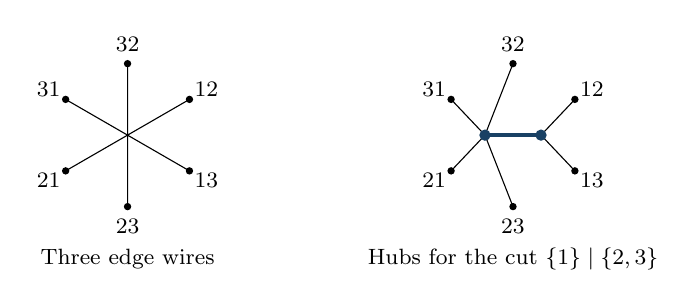
\begin{tikzpicture}[scale=.89, every node/.style={font=\footnotesize}]
\foreach \shift/\layout in {0/0,5.5/1}{
  \begin{scope}[xshift=\shift cm]
    \foreach \p/\angle/\lab in {ab/30/12,ba/210/21,ac/-30/13,ca/150/31,bc/-90/23,cb/90/32}{
      \coordinate (\p) at (\angle:1.02);
      \node at (\angle:1.30) {\lab};
    }
    \ifnum\layout=0
       \draw (ab)--(ba) (ac)--(ca) (bc)--(cb);
       \node at (0,-1.77) {Three edge wires};
    \else
       \coordinate (s) at (.40,0); \coordinate (t) at (-.40,0);
       \draw (ab)--(s)--(ac) (ba)--(t)--(ca) (bc)--(t)--(cb);
       \draw[linkblue,very thick] (s)--(t);
       \fill[linkblue] (s) circle(2.3pt) (t) circle(2.3pt);
       \node at (0,-1.77) {Hubs for the cut \(\{1\}\mid\{2,3\}\)};
    \fi
    \foreach \p in {ab,ba,ac,ca,bc,cb}{\fill (\p) circle(1.5pt);}
  \end{scope}
}
\end{tikzpicture}
\caption{Each label \(ij\) marks the end of edge \(ij\) owned by vertex
\(i\). Moving the hubs apart shortens their spokes in total.}
\label{fig:hubs}
\end{figure}

With both hubs at the origin the spokes have total length \(2m\).
Move them a distance \(t>0\) in opposite directions, the hub of \(S\)
toward \(w_S=v_S/\norm{v_S}\). The distance between hubs becomes \(2t\).
For unit vectors \(u,w\),
\(\norm{u-tw}\le 1-t\inner{u}{w}+t^2/2\), by
\(\sqrt{1+x}\le1+x/2\). The two sides have vector sums \(v_S,-v_S\),
so together their spokes have length at most
\(2m-2t\norm{v_S}+mt^2\).

Fix \(0<t<1\) and use Imported Theorem~\ref{imp:geometry} on the
terminal and hub positions of this drawing. Indices at the same position
are grouped at one site. The scale \(c_t\) is fixed as \(\ell\) grows.
The target has price \(2m\ell\). Each cut network pays \(\ell\) times
its spoke length and \(2t r_\ell\) for its middle wire. Since the
spectral value of the target is at most the sum of those of the cut
networks, its price is at most their largest price plus
\(c_t\log_2|\bal|\). Thus
\[
  2m\ell\le \ell(2m-2t k^{3/2}/3+mt^2)+2t r_\ell+c_t\log_2|\bal|.
\]
Subtract \(2m\ell\) and divide by \(2t\ell\). At fixed \(t\) the last
charge divided by \(2t\ell\) tends to zero, and
\(r_\ell=\lceil\log_2 L_\ell\rceil\). Taking the lower limit gives
\(\beta\ge k^{3/2}/3-mt/2\). Now let \(t\) decrease to zero.
\end{proof}

\section{From wire length to clique size}

Write \(C_F(P)\) for the smallest circuit size of \(P\) over \(F\).
We first fix the clique order and let the host graph grow.

\begin{theorem}
For every field \(F\) and fixed \(k\ge2\),
\[
  \liminf_{N\to\infty}\frac{\log C_F(\Clique_{N,k})}{\log N}
          \ \ge\ \frac{k^{3/2}}{3(k-1)} .
\]
\end{theorem}
\begin{proof}
Set \(N_\ell=k2^{(k-1)\ell}\). By Lemma~\ref{lem:colors}, a circuit
for \(\Clique_{N_\ell,k}\) computes \(Z_{k,2^\ell}\) after substitution,
so it needs at least \(L_\ell\) gates. For \(N_\ell\le N<N_{\ell+1}\),
setting the extra vertex weights to zero gives the same lower bound
at \(N\). Meanwhile \(\log_2 N<\log_2 k+(k-1)(\ell+1)\).
Divide and take the lower limit. Proposition~\ref{prop:wire} gives
the numerator exponent \(k^{3/2}/3\), and the denominator contributes
the factor \(k-1\).
\end{proof}

\begin{corollary}
Over every field \(F\), weighted clique witnesses both
\(\VP_F\subsetneq\VNP_F\) and
\(\mathrm{VFPT}_F\subsetneq\mathrm{VW}[1]_F\).
\end{corollary}
\begin{proof}
A fixed-parameter circuit bound for \(\Clique_{N,k}\) would have the
form \(f(k)N^a\), with the same exponent \(a\) for all \(k\).
Choose \(k\) so that \(k^{3/2}/(3(k-1))>a\), then keep it fixed.
As \(N\) grows, the constant \(f(k)\) disappears from the exponent.
This contradicts the theorem. Appendix~\ref{app:selectors} gives
membership in \(\mathrm{VW}[1]_F\) and the inclusion of \(\mathrm{VFPT}_F\).

For ordinary clique, mark each chosen vertex with a variable \(t\).
The coefficient of \(t^k\) in \(\Clique_N(tX,E)\) is \(\Clique_{N,k}\).
Starting with a circuit for \(\Clique_N\), store the coefficients through
degree \(k\) at every gate. Addition is entry by entry. At a product,
the entry of degree \(d\) is the sum of the products of entries with
degrees \(i\) and \(d-i\), for \(0\le i\le d\). Each gate costs
\(O((k+1)^2)\) operations, over any field. Thus a polynomial bound for
\(\Clique_N\) would give a forbidden bound \(f(k)N^a\) for its parts.
The Boolean sum in Appendix~\ref{app:selectors} puts \((\Clique_N)\)
in \(\VNP_F\), proving the ordinary separation.
\end{proof}

\nocite{anthropic}
\bibliographystyle{../linkedtitles}
\bibliography{../references}


\appendix
\section{Supporting definitions and proofs}

\subsection{Tensor restrictions, covers and spectral points}
\label{app:tensors}

A tensor on a finite set \(I\) of sites is an array with one index for
each site and entries in \(\F\). Use an index of dimension one at an
unused site. A \emph{restriction} applies a linear map to each index
separately. Tensors \(R_1,\ldots,R_j\) \emph{cover} \(T\) if \(T\) is
a sum of one restriction of each \(R_i\). Write \(T\boxtimes R\) for
the tensor product in which the two indices at each site are grouped
as a pair.

A \emph{spectral point} \(\phi\) assigns nonnegative real values to
tensors on \(I\). It takes value one on the scalar unit, is multiplicative
under \(\boxtimes\), and satisfies \(\phi(T)\le\sum_i\phi(R_i)\) for
every cover. A one-term cover gives monotonicity under restriction.
Applying this in both directions shows that invertible local changes
of basis preserve the value.

For the cover inequality, place the source tensors in separate diagonal
blocks at every site (their direct sum). The local maps defining the
cover can act separately on these blocks. Their combined image is the
desired sum. A spectral point adds on direct sums and cannot increase
under local maps, giving the inequality used in the drawing.

\subsection{Summing over subsets}
\label{app:selectors}
For Boolean selectors \(y_1,\ldots,y_N\), take the product
\[
  \prod_i\bigl(1+y_i(X_i-1)\bigr)
  \prod_{i<j}\bigl(1+y_i y_j(E_{ij}-1)\bigr).
\]
A selected vertex contributes \(X_i\). An edge contributes \(E_{ij}\)
exactly when both endpoints are selected. Every other factor is one.
The product has polynomial size and degree. Summing it over all bit
strings gives \(\Clique_N\), as required in the definition of \(\VNP_F\).

For \(\mathrm{VW}[1]_F\) the sum runs over selectors with exactly \(k\)
ones. Each factor above has a bounded-fan-in, constant-depth circuit.
A single product gate combines all factors, so at most one gate of
unbounded fan-in occurs on any path. This is the required weft-one
circuit for the summand, and the sum gives \(\Clique_{N,k}\).%
\sourcenote{Bläser and Engels~\cite{be}, \href{https://arxiv.org/abs/1907.12287}{full version, Section 4}.}
Finally this class allows fixed-parameter substitutions. The weight-one
sum of the expression \(z\) over one selector equals \(z\). Substituting
any family in \(\mathrm{VFPT}_F\) for \(z\) proves the inclusion.

\end{document}
